\documentclass{bioinfo}

%\usepackage{doi}
\usepackage{url}

\copyrightyear{2015}
\pubyear{2015}

\begin{document}
\firstpage{1}

\title[lossy-compression]{Lossy compression of DNA sequencing quality
  data} 
  
\author[Hill \textit{et~al.}]{Christopher M. Hill\,$^{1}$, Andr\'{a}s
  Szolek\,$^{2}$, Mohamed El Hadidi\,$^{3}$, and Michael
  P. Cummings\,$^4$\footnote{to whom correspondence should be
    addressed}} \address{$^{1}$Department of Computer Science,
  University of Maryland, College Park, Maryland, 20742
  USA\\ $^{2}$Department of Applied Bioinformatics, Center for
  Bioinformatics, Quantitative Biology Center, and Department of
  Computer Science, University of T\"{u}bingen, Sand 14, 72076
  T\"{u}bingen, Germany\\ $^{3}$Department of Algorithms in
  Bioinformatics, Center for Bioinformatics, University of
  T\"{u}bingen, Sand 14, 72076 T\"{u}bingen, Germany \\ $^{4}$ Center
  for Bioinformatics and Computational Biology, University of
  Maryland, College Park, Maryland, 20742 USA}

\history{Received on XXXXX; revised on XXXXX; accepted on XXXX}

\editor{Associate Editor: XXXXXXX}

\maketitle

\begin{abstract}

\section{Motivation:}

The \textsc{fastq} file format has become the \emph{de facto} standard
for storing next-generation sequencing data, containing nucleotide
information along with a quantitative measure of the reliability of
individual base calls. As the cost of sequencing continues to
decrease, the rate of sequence data production is increasing,
requiring efficient ways of storing and transferring this vast amount
of data. Most methods of sequencing data compression focus on
compressing nucleotide information without any loss of information.
Quality data, however, have different properties than nucleotide data,
and methods compressing nucleotide sequences efficiently do not
perform as well on quality sequences. Furthermore, while lossless
representation is necessary for nucleotide sequences, it is not an
essential requirement for quality values.

Existing methods for compressing quality sequences mostly focus on
minimizing the loss of information with less emphasis on the effects
on subsequent analyses. In this paper, we evaluate several different
compression methods for quality values that compromise accuracy for
better storage efficiency, and their resulting impact on common
bioinformatic analyses using sequence read data.

\section{Results:}
Lossy compression of quality information can greatly decrease storage
and memory requirements with little discernible effect on subsequent
analysis results. The three compression strategies in this study were
able to produce results similar to those obtained with uncompressed
quality sequences when performing quality control, genome assembly,
and alignment of short reads to a reference sequence.

\section{Contact:} \href{mike@umiacs.umd.edu}{mike@umiacs.umd.edu}
\end{abstract}

\section{Introduction}

Read data from high-throughput sequencing constitutes the largest
category of data in genomics research because of great redundancy,
inclusion of quality values, and read-level naming and
metadata. Because of this abundance, effective compression of read
data has the potential to substantially improve data storage and
transfer efficiency.

Quality values comprise a standard component of \textsc{fastq}
files~\citep{Cock:2010ve}, a very common format for sequence read
data. At the level of the sequence read, the probability of error for
each base-call is typically represented by a \textsc{phred} quality
value, which is defined as $Q =
-10\,log_{10}P$~\citep{Ewing:1998ly}. Depending on the sequencing
technology, these quality values can range from 0 to 93, and are
represented with the \textsc{ascii} characters 33 to 126 (with some
offset). There is a single quality value per base-call for Illumina
sequence reads.

Quality values can be used throughout bioinformatics pipelines. Among
the most fundamental uses of sequence quality values is as part of the
quality assessment and quality control (\textsc{qa/qc}) processes
prior to subsequent analysis steps. Quality control based on quality
values generally includes two operations: \textit{i}.~filtering, which
removes reads that on the whole do not meet arbitrary quality
standards, thus reducing the total number of reads; and
\textit{ii}.~trimming of low-quality base-calls from reads, which
reduces the number total number of bases. Quality values can be used
by genome assembly software to produce better
assemblies~\cite[e.g.,][]{Bryant:2009uq,Gnerre:2011kx}. Short-read
alignment programs, such as Bowtie2~\citep{Langmead:2012rw}, use
quality values to weight mismatches between read and reference
sequences. Software for detecting single nucleotide polymorphisms
(\textsc{snp}s) can use quality values~\cite[e.g.,][]{McKenna:2010bh},
and identified \textsc{snp}s with high-quality calls are deemed more
reliable than those with low-quality calls, particularly in
low-coverage regions.

Previous literature on sequence data compression has largely focused
on lossless compression of base calls~\cite[reviewed
  in][]{Deorowicz:2013hq,Giancarlo:2014rw,Giancarlo:2009fk,
  Nalbantoglu:2010uq,Zhu:2013qr}, although some recent work has
addressed compression of quality
values~\cite[e.g.,][]{asnani2012lossy,Canovas:2014fr,Hach:2012ys,
  janin2013adaptive,Kozanitis:2011kl,Ochoa:2013rt,Tembe:2010ys,
  Wan:2012kq,DBLP:conf/recomb/YuYB14,zhou2014compression}. Among the
several challenges for compression of read data is dealing with
different error profiles resulting from differences in underlying
chemistries, signal detection and processing mechanisms, inherent
biases, and other idiosyncratic properties of distinct high-throughput
sequencing technologies. Sequence reads generated by instruments such
as an Illumina HiSeq, the focus of this research due to its
ubiquitousness in bioinformatics research, are characterized by having
relatively few insertion and deletion errors, but substitution
(miscall) errors are much more frequent and have context-specific
patterns. These errors are non-uniformly distributed over the read
length (e.g., error rates increase up to $\sim$16$\times$ at the
3$^{\prime}$ end, and 32.8 -- 67.9\% of reads have low-quality tails
at the 3$^{\prime}$ end~\citep{Minoche:2011km}).

Although we recognize the need for lossless compression for some
purposes and contexts (e.g., archiving, provenance), our perspective
is largely pragmatic with a focus on the use of quality values in
subsequent analyses. From this perspective, some loss of information
is deemed acceptable if the inferences from analyses are relatively
unaffected. Here we describe our research investigating lossy
compression of sequence read quality values, specifically those
associated with Illumina instruments, with the objective to provide
some perspective on several strategies rather than to develop robust
high-quality software for use. Recognizing these properties of
Illumina sequence reads motivates our exploration of three general
classes of lossy compression methods -- binning, modeling, and
profiling -- and our consideration of an exemplar of each
class.~\cite{Canovas:2014fr} and~\cite{janin2013adaptive} evaluated
the effects of lossy compression on identifying variants within a data
set. We build on these prior works, and assess the effects of quality
value information loss resulting from compression on subsequent
genomic analyses, including read preprocessing (filtering and
trimming), genome assembly, and read mapping.

\begin{methods}
\section{Methods}

\subsection{Compression strategies}

\subsubsection{Binning}

Quality values can be binned, and the minimum number of bins that
allows for a any distinction among quality values is two; i.e., two
categories of quality: ``good'' and ``bad''. We implement 2-bin
encoding by setting a quality value threshold empirically determined
by the distribution of quality values across reads. Base-calls are
marked ``bad'' if their quality value falls below the first quartile
minus 1.5 $\times$ the interquartile range (IQR), which is the
difference between the first and third quartile. 1.5 $\times$ IQR is
the value used by Tukey's box plot~\citep{mcgill1978variations}. The
main benefit of this approach is that it is completely data-dependent,
and no assumptions regarding the distribution of the quality values
need to be made.
 
With 2-bin encoding, binary encoding is possible, allowing us to use a
single bit to represent the quality of a base instead of the standard
8 bits used to store quality values in \textsc{ascii}. An additional
benefit of 2-bin encoding is the potential for increased adjacency of
identical values and repeating patterns, properties that may increase
effectiveness of subsequent compression using established
algorithms~\cite[e.g.,][]{HUFFMAN:1952nr,Ziv77auniversal,
  DBLP:journals/tit/ZivL78}.

The economic costs of memory use for binning, in general terms,
include no fixed costs, and marginal costs that are a function of the
number of base-call quality values times the cost of the encoding.

\cite{Wan:2012kq} provide three similar lossy compression strategies
based on binning the base error probability distribution: UniBinning,
Truncating, and LogBinning. UniBinning evenly splits the error
probability distribution into a user-defined number of partitions.
Truncating treats a user-defined number of highest quality values as a
single bin. LogBinning works similarly to UniBinning, except it uses
the \emph{log} of the error probability distribution, which
effectively bins the \textsc{ascii} quality values evenly. Our 2-bin
encoding is a combination of LogBinning and Truncating in that we
place the highest quality values (as defined above) of the log of the
error probability distribution into a single bin.

\begin{figure}[!tpb]
\centerline{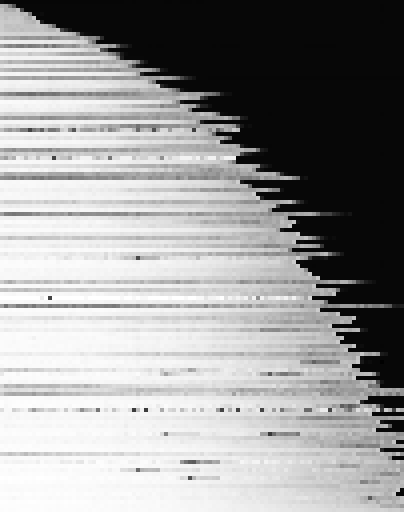
\includegraphics[width=3.35in]{profiles_128.png}}
\caption{Quality profiles obtained by $k$-means clustering on the
  fragment library from \textit{Rhodobacter sphaeroides} 2.4.1 data
  set using $k$ = 128, with each row corresponding to a quality
  profile. Dark to light colors represent low to high quality
  values. It is readily visible that the two most distinctive features
  of quality profiles is their drop-off position and average overall
  quality. One can also see sporadic low-position values in a handful
  of profiles, likely capturing intermittent problems in the
  sequencing process affecting thousands of reads at a
  time.}\label{fig:profiles_128}
\end{figure}

While we focus only on two bins in this work, a greater number of bins
can be used in practice. For example, an additional third bin (good,
bad, and \emph{okay}) can be used for base qualities near the border
between bins in the 2-bin encoding. Examining the trade-off of
additional bins and their resulting compressibility and effect on
downstream analyses is outside the scope of this work.

\subsubsection{Modeling}

If quality values are modeled, compression is conceivably possible by
replacing the original quality values by a representation of the
model. For example, quality values can be conceptualized as bivariate
data with the ordered nucleotides (1 to read length) representing the
abscissa, and quality values representing the ordinate. We model read
quality values as polynomial functions obtained with least-squares
fitting, as one approach to the compression of read quality values by
modeling.  Although polynomial functions have significantly fewer
parameters than a read-length string of raw quality values (e.g., one
to six coefficients in our approach), the use of floating point
numbers to store coefficients greatly limits the compression potential
of the method. The coefficients could be represented with fewer bits,
perhaps with some loss of precision, but we have not considered
alternative representations in this study.

The economic costs of memory use for model-based compression, in
general terms, include no fixed costs, and marginal costs that are a
function of the number of reads times the cost of representing the
model parameters.

\subsubsection{Profiling}

Sets of quality strings show similar trends of quality over their
length, and it is possible to identify common patterns in the data and
use them as reference profiles to approximate individual sequences of
quality values. Here we use $k$-means clustering, a vector
quantization method that partitions a set of samples into $k$ sets
that minimize within-cluster sum of
squares~\citep{macqueen1967some}. We sampled 10$K$ reads at random and
computed cluster centers as read quality profiles using a heuristic
iterative refinement approach that quickly converges to a locally
optimal minimum~\citep{hartigan1979algorithm}.  All reads are
evaluated with the nearest quality profile in Euclidean space being
assigned to every read as their compressed representation.  The
compressed quality file therefore consists of an index enumerating the
$k$ quality profiles, and a binary part containing the assigned
quality profile index for each read.  Although this approach is not
able to capture some read-specific differences in quality values, it
does approximate the overall patterns in quality values. An example of
128 quality profiles is shown in Figure \ref{fig:profiles_128}.

The economic costs of memory use for profile-based compression, in
general terms, include fixed costs associated with representing the
profiles, which is a function of the number of profiles times the cost
of encoding them, and these fixed costs are amortized over the entire
set of reads to which they apply. Additionally there are marginal
costs that are a function of the number of reads encoded.

Profiles can be obtained from techniques other than $k$-means
clustering. We can store the profiles of polynomial functions to
increase the compressibility of polynomial regression modeling.  In
other words, we can use a spline (a function that is piecewise-defined
by polynomial functions) to represent a given quality sequence.
However, we have not explored any of these other approaches here.

\subsection{Data sets}

We used several Illumina sequence read data sets in this research,
which are taken from data from the \textsc{gage} (Genome Assembly
Gold-Standard Evaluations)~\citep{Salzberg:2012rc}, except as
noted. These data sets are as follows.

\textit{Rhodobacter sphaeroides} 2.4.1, which are generated from a
fragment library (insert size of 180 nt; 2,050,868 paired-end reads)
and short-jump library (insert size of 3,500 nt; 2,050,868 reads). The
corresponding reference sequence was obtained from the \textsc{ncbi}
RefSeq database (NC\_007488.1, NC\_007489.1, NC\_007490.1,
NC\_007493.1, NC\_007494.1, NC\_009007.1, NC\_009008.1).

\textit{Homo sapiens} chromosome 14 data, which are generated from a
fragment library (insert size of 155 nt; 36,504,800 paired-end reads)
and short-jump library (insert sizes ranging from 2283-2803 nt;
22,669,408 reads). The corresponding reference sequence was obtained
from the \textsc{ncbi} RefSeq database (NC\_000014.8).

\textit{Escherichia coli} str. K-12 MG1655 MiSeq data was downloaded
from \url{http://www.illumina.com/systems/miseq/scientific_data.html},
which are generated from a fragment library (insert size of 180bp nt;
1,145,8940 paired-end reads). The corresponding reference sequence was
obtained from the \textsc{ncbi} RefSeq database (NC\_000913.2).

\textit{Mus musculus} data was downloaded from
\url{http://trace.ddbj.nig.ac.jp/DRASearch/run?acc=SRR032209}, which
consisted of 18,828,274 reads of length 36.

\subsection{Comparison to other methods}

For comparison to other developed methods we use \textsc{QualComp}, a
lossy compression tool~\citep{Ochoa:2013rt}. The program models
quality values as a multivariate Gaussian distribution, computing the
mean and covariance for each position in the read, and these varlues
are stored by the decoder to later reconstruct a \emph{representative}
quality value. \textsc{QualComp} takes as input a user-specified rate
(bits/read), and these bits are allotted among positions within the
read to minimize the average error. The quality values can be
clustered beforehand to produce more accurate models.

\subsection{Performance evaluation}

As a measure of compression effectiveness we use bits/base-call, and
define it as the size of the compressed representation of quality
values (in bits) divided by the number of quality values represented.
As a measure of information loss we use mean squared error
(\textsc{mse}) as a loss function, and define it as
$\frac{1}{n}\sum_{i=1}^{n}{(Q_i'-Q_i)^2}$, where $n$ is the number of
sequences, $Q_i'$ is the compressed/decompressed quality value, and
$Q_i$ is the original quality value associated with sequence position
$i$.

We evaluate effects of information loss from quality value compression
on quality control steps of trimming and read filtering, which were
performed using Sickle~\citep{sickle}, and make comparison to
uncompressed data. Sickle starts at the ends of the read and uses a
sliding window ($0.1 \times$ the read length) to find locations where
the mean quality in the window falls below a given threshold (20 by
default). The sequence is then trimmed from this position to the
respective end. If the trimmed sequence length is less than a certain
threshold (20 by default), then the sequence is discarded.

We evaluate effects of information loss from quality value compression
on \emph{de novo} genome assembly performance using contiguity
statistics, log average read probability
(\textsc{lap})~\citep{Ghodsi:2013hb}, and a collection of
reference-based metrics. The contiguity statistics include N50, which
is defined as the median contig size (the length of largest contig $c$
such that the total size of the contigs larger than $c$ exceeds half
of the assembly size) and corrected N50, which is the recalculated N50
size after the contigs are broken apart at locations of errors. The
\textsc{lap} score can be viewed as a log-likelihood score, where a
value closer to 0 is better. We use a script provided by \textsc{gage}
reference-based evaluation to count single nucleotide polymorphisms
(\textsc{snp}s), relocations, translations, and inversions. The
reference-based metrics are normalized by the length of the assembly
to facilitate comparison. For the genome assembly we used software
that makes use of quality values in the assembly process:
\textsc{allpaths-lg}~\citep{Gnerre:2011kx} version r50191 with default
settings and 32 threads.

\end{methods}

\section{Results}

\subsection{Compression effectiveness versus information loss}

\begin{figure*}[!tb]
\centerline{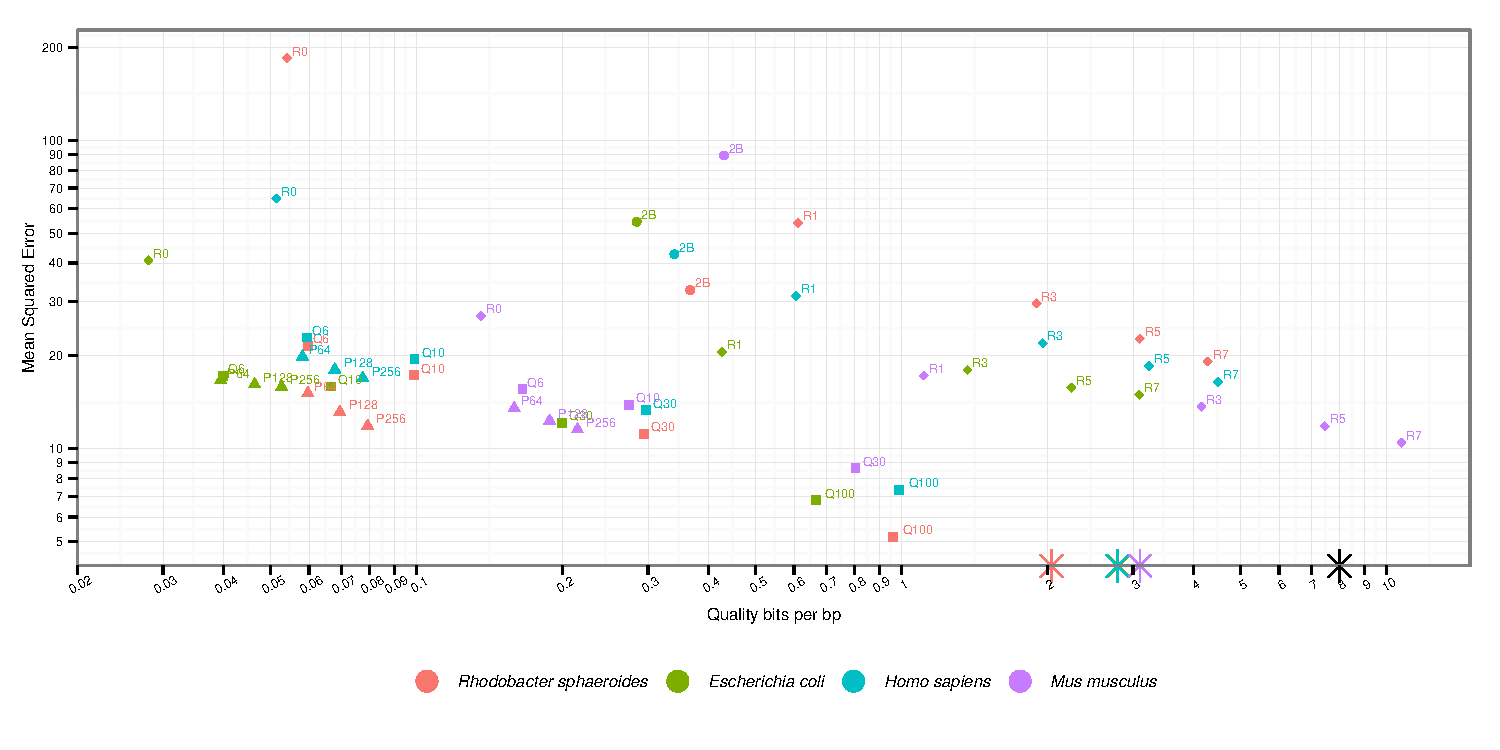
\includegraphics[width=7in]{compression_results.pdf}}
\caption{The relationship of bits/base-call and mean squared error for
  quality value compression methods applied to four data sets:
  \textit{Rhodobacter sphaeroides} 2.4.1; \textit{Homo sapiens}
  chromosome 14; \textit{Escherichia coli} str. K-12 MG1655; and
  \textit{Mus musculus}. Point labels correspond to different
  compression methods: 2B, 2-bin encoding; P$n$, profiling with $n$
  profiles; R$n$, modeling with polynomial regression of degree $n$;
  Q$n$, \textsc{q}ual\textsc{c}omp with rate parameter of
  $n$. Asterisks denote the corresponding lossless compression using
  \textsc{bz}ip2, with the black asterisk corresponding to original
  data.}
\label{fig:mse_vs_bpbp}
\end{figure*}

We compare the \textsc{mse} versus bits/base-call of the
\textit{Rhodobacter sphaeroides}, \textit{Homo sapiens},
\textit{Escherichia coli}, and \textit{Mus musculus} data sets (Figure
\ref{fig:mse_vs_bpbp}). Here we present the fragment libraries for the
\textit{Rhodobacter sphaeroides}, and \textit{Homo sapiens} data sets,
but the short-jump library results are available in Supplemental Table
1. Storing the uncompressed quality values requires 1 byte/base-call
because they are stored in \textsc{ascii} format, which is denoted by
the dotted black asterisk in the figure. The lossless compression of
each data set using \textsc{bz}ip2 ranges from 2.19--3.10
bits/base-call and is denoted by the colored asterisks on the
abscissa. The compression methods tend to cluster together across the
different data sets. Across all data sets, the 0-degree polynomial
regression, profile encodings, and \textsc{q}ual\textsc{c}omp have the
lowest bits/base-call.

\textsc{q}ual\textsc{c}omp with the rate parameter set to 100
bits/read has the lowest \textsc{mse}, but requires
$\sim$10--15$\times$ more storage than the profile encoding methods
for only a $\sim$2--3$\times$ reduction in \textsc{mse}. When rate
parameter of \textsc{q}ual\textsc{c}omp is set to match the profile
encoding methods, \textsc{q}ual\textsc{c}omp performs slightly worse
in terms of \textsc{mse}. For the \textit{Rhodobacter sphaeroides}
fragment library, \textsc{q}ual\textsc{c}omp with rate set to 10
bits/read (0.099 bits/bp) has a \textsc{mse} of 17.29, whereas
256-profile encoding only requires 0.079 bits/bp and has a
\textsc{mse} of 11.85.

As the degree of the polynomial increases, the bits/base-call increase
and the \textsc{mse} decreases at an exponential rate. The 7th-degree
polynomial regression has the highest bits/base-call in the
\textit{Mus musculus} data set, and requires more storage than the
original \textsc{ascii} quality values. A 7th-degree polynomial
requires storing eight floating point values, resulting in 32 bytes
per sequence of quality values. The read length of the \textit{Mus
  musculus} data set is only 26, so the 7th-degree polynomial
regression is storing six more bytes than necessary for lossless
encoding of the quality data.

As an additional point of reference regarding compression
effectiveness, the recently published
Read-Quality-Sparsifier~\citep{DBLP:conf/recomb/YuYB14} achieved
best-case compression of 0.254 bits/base-call, and a mean compression
of 1.841 bits/base-call; both values are higher than all of the
profile results and for some results of other methods presented here
(Figure~\ref{fig:mse_vs_bpbp}).

\subsection{Effects on sequence read preprocessing}

Preprocessing involves two steps: \emph{trimming} the poor-quality
regions of the sequences, and \emph{discarding} sequences that are
deemed to be poor-quality overall. After trimming, the majority of
compression methods retain more base-pairs than the uncompressed
sequences (Figure \ref{fig:preprocessing}). In general, as a given
compression model increases in complexity --- i.e., as the number of
profiles, polynomial degrees, or rate increases --- the amount of
base-pairs kept approaches the number of base-pairs kept using the
uncompressed sequences. The compression methods on the \textit{Mus
  musculus} data set have the greatest proportion of retained
base-pairs compared to the uncompressed sequences. The
\textit{Escherichia coli} MiSeq data set has the smallest range.

The 2-bin approach is the only compression method that results in a
higher number of trimmed base-pairs across all data sets. Sickle uses
a sliding window approach to smooth the read quality values before it
trims. In the 2-bin approach, there is not an even distribution of
values per bin. In other words, \emph{bad} quality values may range
from 0--33, whereas \emph{good} values may only range from
34--40. Thus, mid-range quality values that are above the threshold
(20 by default) are set below the quality threshold when compressed,
resulting in an increased number of trimmed bases.

The 0-degree polynomial regression results in the highest proportion
of bases kept. If the mean quality value of the read is above the
filtering threshold, then no base-pairs are trimmed. Only reads that
are comprised of mainly low quality values will be discarded.

It is important to highlight that even though a compression method may
result in the same number of trimmed bases as the uncompressed
sequences, it does not mean the \emph{same} bases were trimmed. The
1st-degree and 5th-degree polynomial regression of the
\textit{Rhodobacter sphaeroides} fragment library filter nearly as
many bases as each other. However, if we examine the specific reads
discarded, the 5th-degree polynomial regression discards approximately
two-thirds less reads than the 1st-degree polynomial regression that
are kept by the uncompressed reads (4,640 and 12,066 reads,
respectively) (Supplemental Table 2).

\begin{figure}[!tbp]
\centerline{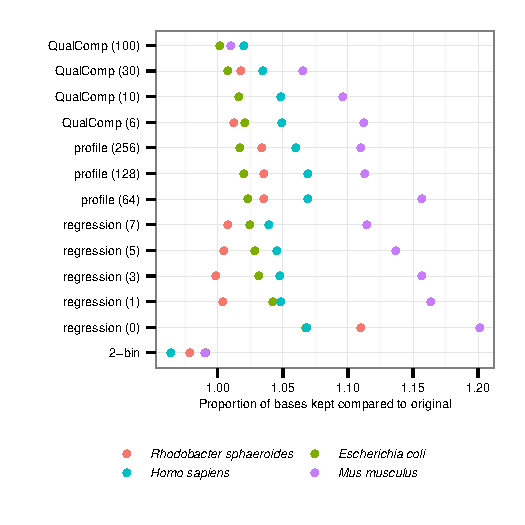
\includegraphics[width=3.65in]{preprocessing_results.pdf}}
\caption{Preprocessing results of \textit{Rhodobacter sphaeroides}
  2.4.1, and \textit{Homo sapiens} chromosome 14 fragment libraries,
  and \textit{Escherichia coli} str. K-12 MG1655, and \textit{Mus
    musculus} data sets. Sequences were trimmed using Sickle. The
  total amount of bases filtered by each compression method is
  compared with the amount of bases filtered using the uncompressed
  sequences.}
  \label{fig:preprocessing}
\end{figure}

\subsection{Effects on genome assembly}

No assembly of the \textit{Rhodobacter sphaeroides} data set was best
in all metrics (Table \ref{fig:assembly_ranks}). Among the compression
methods, the profile encoding performed best, polynomial regression
modeling performed worst, and other methods were intermediate
(Fig.~\ref{fig:assembly_ranks}).

The lossy compression methods largely preserve the contiguity found in
the assembly produced using the reads with unmodified quality
values. All compression methods other than 0-degree polynomial
regression produce an N50 ranging from 3.17--3.22 Mbp (see
Supplemental Table 3). Despite the similar contiguity statistics, the
different compression methods vary noticeably in the amount of
\textsc{snp}s. The 2-bin and profile methods exhibited the fewest
\textsc{snp}s compared to the reference genome, thus outperforming the
assembly using the original quality values in this characteristic. A
more in-depth evaluation is needed to determine whether these
compression methods are missing actual \textsc{snp}s.

It is important to highlight that using uncompressed reads does not
produce the best assembly in terms of any of the metrics. The
uncompressed reads score worse than the top overall assembly
(256-profile encoding) in terms of assembled bases, missing reference
bases, N50, \textsc{snp}s, indels $>$5bp, and relocations. The
assembly using the original uncompressed reads has an error rate of
roughly 8.75 errors per 100 kb of assembled sequence, while the
256-profile encoding has an error rate of 8.02 errors per 100 kbp
(Supplemental Table 3).

In general, the greater the polynomial degree, the better the overall
assembly; however, the 5th-degree polynomial regression performs
slightly worse than the 3rd-degree polynomial. The respective ranks in
terms of N50 and relocations are fairly distant, which lowers the
overall ranking of the 5th-degree polynomial slightly below that for
3rd-degree polynomial model. The 1st- and 0-degree polynomial
regression methods perform poorly in all metrics except assembled
bases. One explanation is that the high-error portions of reads are
being marked as high quality, so \textsc{allpaths-lg} is unable to
trim or error-correct the sequences. Assembled sequences that overlap
may be unable to align across the errors at the end of the reads,
artificially inflating the assembled genome size.

Among the different \textsc{q}ual\textsc{c}omp rate parameters, the 10
bits/read rate ranked highest overall, outperforming the other rate
parameters in terms of corrected N50, fewest missing reference bases,
\textsc{snp}s, and indels $>$5bp. With the exception of the 6
bits/read rate, the assemblies decrease in rank with the increase in
the rate parameter in terms of corrected N50, and fewest missing
reference bases. This trend runs counter to the decrease in
\textsc{mse} of the different rates.

\begin{figure}[!tbp]
\centerline{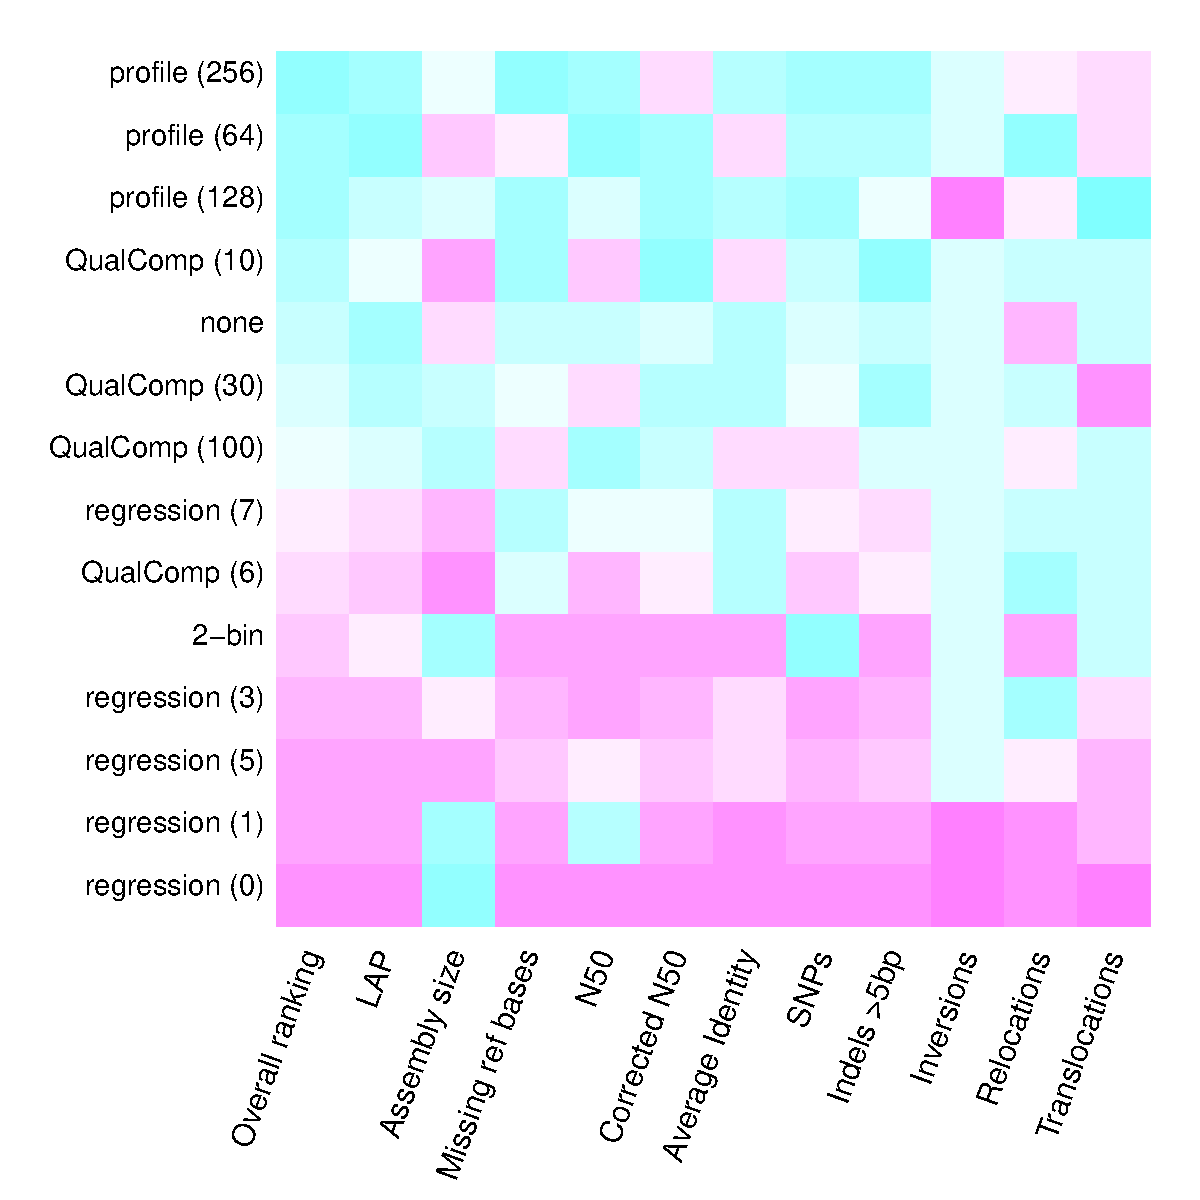
\includegraphics[width=3.65in]{rhodo_assembly_results.pdf}}
\caption{Rankings of compression methods based on \textit{Rhodobacter
    sphaeroides} assembly attributes sorted by overall
  rank. Assemblies were constructed using \textsc{allpaths-lg}.
  Rankings above the median value are in cyan, those below the median
  value in magenta.}
  \label{fig:assembly_ranks}
\end{figure}

\begin{table*}[!tbhp]
\centering
\caption[]{Comparison of mapping for original reads and reads with
  compressed/decompressed quality values. Reads and reference genome
  are for \textit{Rhodobacter sphaeroides}, and mapping was performed
  using Bowtie2.}
\begin{small}
\begin{tabular}{lr|cc|cc|cc|cc|cc}
 & & \multicolumn{2}{c|}{max-qual} & \multicolumn{2}{c|}{min-qual} & \multicolumn{2}{c|}{2-bin} & \multicolumn{2}{c|}{regression (0)} & \multicolumn{2}{c}{regression (1)} \\
& & mapped & unmapped & mapped & unmapped & mapped & unmapped & mapped & unmapped & mapped & unmapped \\ 
\cline{2-12}
& mapped & 746716 & 145897 & 892613 &   0 & 891864 & 749 & 851682 & 40931 & 883390 & 9223 \\ 
{\em original} & unmapped &   0 & 132821 & 10821 & 122000 & 186 & 132635 &  67 & 132754 &  55 & 132766 \\ 
\cline{2-12}
& proportion & 0.728 & 0.272 & 0.881 & 0.119 & 0.870 & 0.130 & 0.831 & 0.169 & 0.862 & 0.138 \\ 
\end{tabular}

\bigskip

\begin{tabular}{lr|cc|cc|cc|cc|cc}
 & & \multicolumn{2}{c|}{regression (3)} & \multicolumn{2}{c|}{regression (5)} & \multicolumn{2}{c|}{regression (7)} & \multicolumn{2}{c|}{profile (64)} & \multicolumn{2}{c}{profile (128)} \\
& & mapped & unmapped & mapped & unmapped & mapped & unmapped & mapped & unmapped & mapped & unmapped \\ 
\cline{2-12}
& mapped & 889537 & 3076 & 891019 & 1594 & 891479 & 1134 & 891753 & 860 & 891952 & 661 \\ 
{\em original} & unmapped & 117 & 132704 & 155 & 132666 & 154 & 132667 & 144 & 132677 & 143 & 132678 \\ 
\cline{2-12}
& proportion & 0.868 & 0.132 & 0.869 & 0.131 & 0.870 & 0.130 & 0.870 & 0.130 & 0.870 & 0.130 \\ 
\end{tabular}

\bigskip

\begin{tabular}{lr|cc|cc|cc|cc|cc}
&  & \multicolumn{2}{c|}{profile (256)} & \multicolumn{2}{c|}{\textsc{q}ual\textsc{c}omp (6)} & \multicolumn{2}{c|}{\textsc{q}ual\textsc{c}omp (10)} & \multicolumn{2}{c|}{\textsc{q}ual\textsc{c}omp (30)} & \multicolumn{2}{c}{\textsc{q}ual\textsc{c}omp (100)} \\
& &  mapped & unmapped & mapped & unmapped & mapped & unmapped & mapped & unmapped & mapped & unmapped \\ 
\cline{2-12}
& mapped & 892051 & 562 & 891375 & 1238 & 891777 & 836 & 892233 & 380 & 892454 & 159 \\ 
{\em original}  & unmapped & 119 & 132702 & 304 & 132517 & 265 & 132556 & 220 & 132601 & 172 & 132649 \\ 
\cline{2-12}
& proportion & 0.870 & 0.130 & 0.870 & 0.130 & 0.870 & 0.130 & 0.870 & 0.130 & 0.870 & 0.130 \\
\end{tabular}
\end{small}

\label{tab:aligner}
\end{table*}


\subsection{Effects on read mapping}

Certain short read alignment tools use the quality value information
when finding potential alignments. Bowtie2 (version 2.2.3) was used to
evaluate the different decompressed \textsc{fastq} files. Bowtie2 uses
quality values written in the \textsc{fastq} files when mapping reads
against a reference genome. The original uncompressed and decompressed
\textsc{fastq} files were mapped with Bowtie2 against the
\textit{Rhodobacter sphaeroides} reference genome. The generated
\textsc{sam} file for each compression approach was compared with the
uncompressed \textsc{sam} file. The total, shared and unique
proportional numbers of mapped reads are calculated with respect to
the uncompressed \textsc{sam} matches as shown in Table
\ref{tab:aligner}. Additionally, to monitor the effect of quality
values on mapping in general, Bowtie2 was adjusted so that the maximum
and minimum mismatch penalty were equivalent to maximum and minimum
quality scores (with parameters: --mp 6,6 and --mp 2,2 respectively).

We evaluate the compression methods using two approaches. In the first
approach, we order the compression methods based on how similar the
alignment results are using the original uncompressed quality values
--- i.e., the amount of reads aligned by both the uncompressed and
compressed methods plus the amount of reads unaligned by both methods
minus the amount of reads uniquely aligned by the uncompressed and
compression method. In the second approach, we order the compression
methods by total proportion of aligned reads.

The best compression method in terms of similarity with the
uncompressed reads is \textsc{q}ual\textsc{c}omp with rate 100
bits/read, followed by \textsc{q}ual\textsc{c}omp with rate 30
bits/read, 256-profile encoding, 128-profile encoding, 2-bin encoding,
64-profile encoding, \textsc{q}ual\textsc{c}omp with rate 10
bits/read, 7th-degree polynomial regression,
\textsc{q}ual\textsc{c}omp with rate 6 bits/read, and finally,
5th-degree through 0-degree polynomial regression.

Ranking the compression methods by overall alignment rate produces an
identical ordering as above. Aside from 0-degree polynomial regression
(83.1\%), all other compression methods have an alignment rate between
87\% and 86.1\%. The alignment rate of the uncompressed reads is 87\%.

Most of the compression methods did not vary greatly in terms of the
number of reads that were mapped \emph{only} by the compression
method; however, there is a sizable difference in the amount of reads
that are originally mapped, but unmapped by the compressed methods.
\textsc{q}ual\textsc{c}omp with rate 100 bits/read results in the
fewest missing original read alignments (159). Increasing the
regression model polynomial degree results in a decreasing amount of
reads that are originally mapped, but unmapped by the regression model
(40,931 to 1,134 reads for 0-degree and 7th-degree,
respectively). There is no such trend for reads that are mapped only
by the regression model.

Note that the 2-bin method aligns a greater portion of reads than the
various regression models. If a poor-quality base is flanked by
high-quality sequence, then the low-degree polynomial regression
models tend to smooth out the base quality, erroneously marking the
low-quality base as higher quality.  During alignment, Bowtie2
penalizes mismatches at high-quality bases more so than mismatches at
lower-quality bases. Thus, the polynomial regression models incur a
high penalty for these bases, resulting in fewer alignments, despite
having a better \textsc{mse} than 2-bin in most cases.

Setting all bases as minimum quality results in the highest proportion
of mapped reads (88.1\%). Conversely, setting all bases as maximum
quality results in the lowest proportion of mapped reads (72.8\%).

\section{Discussion}

\subsection{Lossy compression is acceptable for some subsequent  
analyses}

It is common to evaluate lossy compression methods in terms of
information loss, and some measure of compression effectiveness.
However, from a pragmatic perspective, it is the effects on the
results of subsequent analyses that are most important. Our results
showed that some of the compression methods with relatively high
information lossy (\textsc{mse}) are still practical for some
applications. Many bioinformatics tools proved to be robust to
moderate information loss. Passing the decompressed quality values
through quality control software shows that most methods filter nearly
as many bases as using original quality sequences. Assemblers
performing sequence alignment use percent similarity scores that are
typically robust to standard sequencing errors.

Downstream applications dictate which lossy compression methods are
acceptable. As noted above, 2-bin encoding is able to retain
information about low-quality bases that occur within stretches of
high-quality bases, whereas the polynomial regression methods tend to
smooth these qualities. In addition to aligning fewer reads than the
2-bin encoding, the polynomial regression methods may also be
hindering downstream tools that use the alignment results. A
\textsc{snp} detection pipeline will commonly use the quality values
to record if a potential difference from the reference is the result
of genetic variation or sequencing error. Erroneously marking a base
as higher quality may lead to the base being incorrectly labeled as a
\textsc{snp}. 2-bin encoding is acceptable for alignment; however, it
performs quite poorly in terms of assembly, and 7th-degree polynomial
regression modeling outperforms it in nearly all metrics.

\subsection{Potential for operations on compressed data}

Perhaps one of the greatest potential benefits of compressing quality
values is the ability to perform quality control and possibly other
operations directly on the compressed representations of the data. For
example, with profile-based compression, the $k$ profiles can be
evaluated for (pre-)processing operations such as filtering and
trimming, and the operations transitively applied to the entire set of
reads, thus saving substantial computation.

%%%%%%%%%%%%%%%%%%%%%%%%%%%%%%%%%%%%%%%%%%%%%%%%%%%%%%%%%%%%%%%%%%%%%%%%%%%%%%%%%%%%%
%
%     please remove the " % " symbol from \centerline{\includegraphics{fig01.eps}}
%     as it may ignore the figures.
%
%%%%%%%%%%%%%%%%%%%%%%%%%%%%%%%%%%%%%%%%%%%%%%%%%%%%%%%%%%%%%%%%%%%%%%%%%%%%%%%%%%%%%%

\section{Conclusion}

In this paper we have examined several general approaches for lossy
compression of sequence quality values and their effect on subsequent
analyses. Although most previous examinations of lossy compression
focused primarily on information loss and compression effectiveness,
we show that common bioinformatic analyses are robust to substantial
loss of information in quality values.

\section{Availability}
Implementations of the compression methods written in Python and R,
and a pipeline to reproduce the results are available at
\url{https://github.com/cmhill/q-compression}

\section*{Acknowledgement}
This research was initiated at the 2014 Bioinformatics Exchange for
Students and Teachers (\textsc{best}) Summer School, which was funded
by the offices of the Dean of The Graduate School at University of
Maryland and the Rektor of University of T\"{u}bingen.

\bibliographystyle{natbib}
\bibliographystyle{achemnat}
\bibliographystyle{plainnat}
\bibliographystyle{abbrv}
\bibliographystyle{bioinformatics}
%
\bibliographystyle{plain}
%

\bibliography{compression}

\end{document}
